\chapter{Specifications of the STM32F405 and the LIS3DH}
\label{ann:memories_maps}

The Table \ref{tab:lis3dh_registers} provides a list of the 8-bit registers embedded in the LIS3DH 
accelerometer and the corresponding addresses.

\begin{table}[H]
    \centering
    \footnotesize
    \setlength{\tabcolsep}{4pt}
    \renewcommand{\arraystretch}{0.9}
    \begin{tabular}{l c c c c c l}
        \toprule
        \textbf{Name} & \textbf{Type} & \multicolumn{2}{c}{\textbf{Register Address}} & \textbf{Default} & \textbf{Comment} \\
        \cmidrule(lr){3-4}
        & & \textbf{Hex} & \textbf{Binary} & & \\
        \midrule
        \textit{Reserved (do not modify)} & & 00-06 \\
        STATUS\_REG\_AUX    & r     & 07    & 0000 0111  & —         & Output    \\
        OUT\_ADC1\_L        & r     & 08    & 0000 1000  & —         & Output    \\
        OUT\_ADC1\_H        & r     & 09    & 0000 1001  & —         & Output    \\
        OUT\_ADC2\_L        & r     & 0A    & 0000 1010  & —         & Output    \\
        OUT\_ADC2\_H        & r     & 0B    & 0000 1011  & —         & Output    \\
        OUT\_ADC3\_L        & r     & 0C    & 0000 1100  & —         & Output    \\
        OUT\_ADC3\_H        & r     & 0D    & 0000 1101  & —         & Output    \\
        \textit{Reserved (do not modify)} & & 0E                                \\
        WHO\_AM\_I          & r & 0F & 000 1111 & 00110011 & Dummy register     \\
        \textit{Reserved (do not modify)} & & 10 — 1D                          \\
        CTRL\_REG0          & rw    & 1E    & 0001 1110  & 00010000  & —         \\
        TEMP\_CFG\_REG      & rw    & 1F    & 0001 1111  & 00000000  & —         \\
        CTRL\_REG1          & rw    & 20    & 0010 0000  & 00000111  & —         \\
        CTRL\_REG2          & rw    & 21    & 0010 0001  & 00000000  & —         \\
        CTRL\_REG3          & rw    & 22    & 0010 0010  & 00000000  & —         \\
        CTRL\_REG4          & rw    & 23    & 0010 0011  & 00000000  & —         \\
        CTRL\_REG5          & rw    & 24    & 0010 0100  & 00000000  & —         \\
        CTRL\_REG6          & rw    & 25    & 0010 0101  & 00000000  & —         \\
        REFERENCE           & rw    & 26    & 0010 0110  & 00000000  & —         \\
        STATUS\_REG         & r     & 27    & 0010 0111  & —         & Output    \\
        OUT\_X\_L           & r     & 28    & 0010 1000  & —         & Output    \\
        OUT\_X\_H           & r     & 29    & 0010 1001  & —         & Output    \\
        OUT\_Y\_L           & r     & 2A    & 0010 1010  & —         & Output    \\
        OUT\_Y\_H           & r     & 2B    & 0010 1011  & —         & Output    \\
        OUT\_Z\_L           & r     & 2C    & 0010 1100  & —         & Output    \\
        OUT\_Z\_H           & r     & 2D    & 0010 1101  & —         & Output    \\
        FIFO\_CTRL\_REG     & rw    & 2E    & 0010 1110  & 00000000  &           \\
        FIFO\_SRC\_REG      & r     & 2F    & 0010 1111  & —         & Output    \\
        INT1\_CFG           & rw    & 30    & 0011 0000  & 00000000  & —         \\
        INT1\_SRC           & r     & 31    & 0011 0001  & —         & —         \\
        INT1\_THS           & rw    & 32    & 0011 0010  & 00000000  & —         \\
        INT1\_DURATION      & rw    & 33    & 0011 0011  & 00000000  & —         \\
        INT2\_CFG           & rw    & 34    & 0011 0100  & 00000000  & —         \\
        INT2\_SRC           & r     & 35    & 0011 0101  & —         & —         \\
        INT2\_THS           & rw    & 36    & 0011 0110  & 00000000  & —         \\
        INT2\_DURATION      & rw    & 37    & 0011 0111  & 00000000  & —         \\
        CLICK\_CFG          & rw    & 38    & 0011 1000  & 00000000  & —         \\
        CLICK\_SRC          & r     & 39    & 0011 1001  & —         & —         \\
        CLICK\_THS          & rw    & 3A    & 0011 1010  & 00000000  & —         \\
        TIME\_LIMIT         & rw    & 3B    & 0011 1011  & 00000000  & —         \\
        TIME\_LATENCY       & rw    & 3C    & 0011 1100  & 00000000  & —         \\
        TIME\_WINDOW        & rw    & 3D    & 0011 1101  & 00000000  & —         \\
        ACT\_THS            & rw    & 3E    & 0011 1110  & 00000000  & —         \\
        ACT\_DUR            & rw    & 3F    & 0011 1111  & 00000000  & —         \\
        \bottomrule
    \end{tabular}

    \caption{LIS3DH Registers}
    \label{tab:lis3dh_registers}
\end{table}


\newpage

The Figure \ref{fig:stm32f405_i2c} represents the complete mapping of the configuration bits of the I$^2$C peripheral in the STM32F405.

\begin{figure}[H]
    \centering
    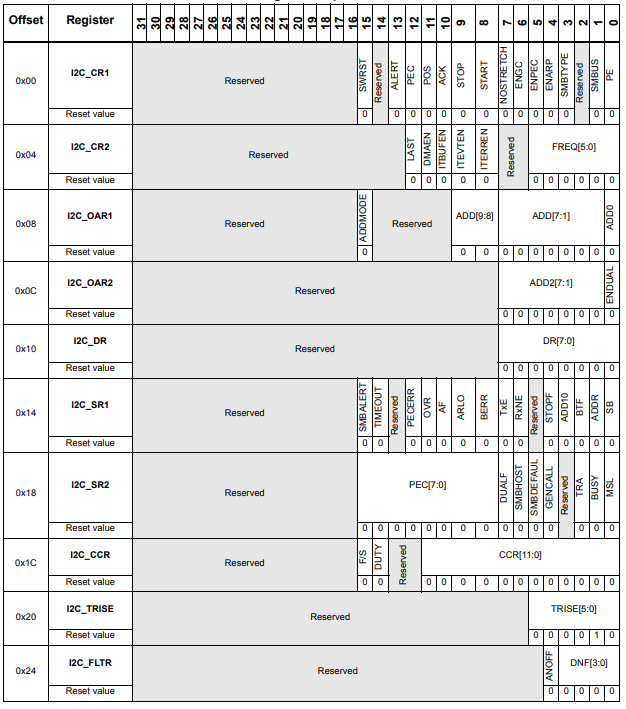
\includegraphics[width=0.95\textwidth]{Resources/Imagenes/stm32f405_i2c.png}
    \caption{stm32f405 i2c memory map}
    \label{fig:stm32f405_i2c}
\end{figure}
